\documentclass[border=10pt]{standalone}
\usepackage{pgfplots}
\usepgfplotslibrary{colormaps}
\pgfplotsset{compat=1.18}

\begin{document}
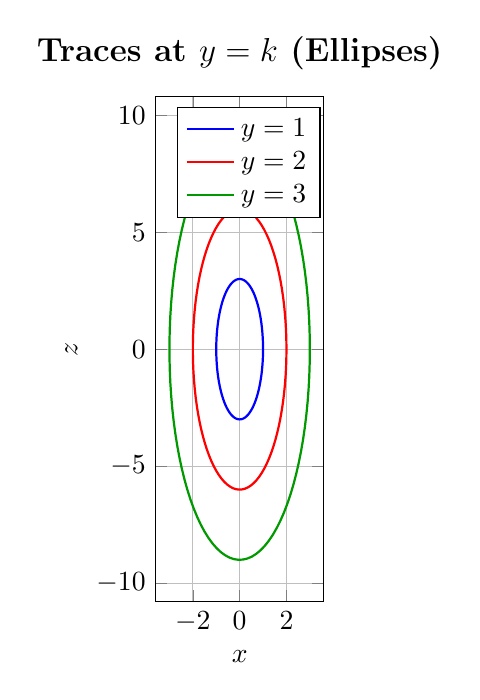
\begin{tikzpicture}
\begin{axis}[
    xlabel={$x$},
    ylabel={$z$},
    title={Traces at $y = k$ (Ellipses)},
    xlabel style={font=\bfseries},
    ylabel style={font=\bfseries},
    title style={font=\bfseries\large},
    grid=major,
    axis equal image,
    width=10cm,
    height=8cm,
    legend style={at={(0.98,0.98)}, anchor=north east}
]
% Ellipse at y = 1: x^2 + z^2/9 = 1
\addplot[domain=0:360, samples=100, thick, blue] ({cos(x)}, {3*sin(x)});
\addlegendentry{$y = 1$}

% Ellipse at y = 2: x^2 + z^2/9 = 4
\addplot[domain=0:360, samples=100, thick, red] ({2*cos(x)}, {6*sin(x)});
\addlegendentry{$y = 2$}

% Ellipse at y = 3: x^2 + z^2/9 = 9
\addplot[domain=0:360, samples=100, thick, green!60!black] ({3*cos(x)}, {9*sin(x)});
\addlegendentry{$y = 3$}

\end{axis}
\end{tikzpicture}
\end{document}